%%%%%%%%%%%%%%%%%%%%%%%%%%%%%%%%%%%%%%%%%%%%%%%%%%%%%%%%%%%%%%%%%%%%%%%%%%%%%%%%
% Template for USENIX papers.
%
% History:
%
% - TEMPLATE for Usenix papers, specifically to meet requirements of
%   USENIX '05. originally a template for producing IEEE-format
%   articles using LaTeX. written by Matthew Ward, CS Department,
%   Worcester Polytechnic Institute. adapted by David Beazley for his
%   excellent SWIG paper in Proceedings, Tcl 96. turned into a
%   smartass generic template by De Clarke, with thanks to both the
%   above pioneers. Use at your own risk. Complaints to /dev/null.
%   Make it two column with no page numbering, default is 10 point.
%
% - Munged by Fred Douglis <douglis@research.att.com> 10/97 to
%   separate the .sty file from the LaTeX source template, so that
%   people can more easily include the .sty file into an existing
%   document. Also changed to more closely follow the style guidelines
%   as represented by the Word sample file.
%
% - Note that since 2010, USENIX does not require endnotes. If you
%   want foot of page notes, don't include the endnotes package in the
%   usepackage command, below.
% - This version uses the latex2e styles, not the very ancient 2.09
%   stuff.
%
% - Updated July 2018: Text block size changed from 6.5" to 7"
%
% - Updated Dec 2018 for ATC'19:
%
%   * Revised text to pass HotCRP's auto-formatting check, with
%     hotcrp.settings.submission_form.body_font_size=10pt, and
%     hotcrp.settings.submission_form.line_height=12pt
%
%   * Switched from \endnote-s to \footnote-s to match Usenix's policy.
%
%   * \section* => \begin{abstract} ... \end{abstract}
%
%   * Make template self-contained in terms of bibtex entires, to allow
%     this file to be compiled. (And changing refs style to 'plain'.)
%
%   * Make template self-contained in terms of figures, to
%     allow this file to be compiled. 
%
%   * Added packages for hyperref, embedding fonts, and improving
%     appearance.
%   
%   * Removed outdated text.
%
%%%%%%%%%%%%%%%%%%%%%%%%%%%%%%%%%%%%%%%%%%%%%%%%%%%%%%%%%%%%%%%%%%%%%%%%%%%%%%%%

\documentclass[letterpaper,twocolumn,10pt]{article}
\usepackage{usenix2019_v3}
\usepackage{algorithmic}
\usepackage{algorithm}
\usepackage{listings}
\usepackage{pifont}
\usepackage{multirow}
\usepackage{graphicx}
\usepackage{caption}
\usepackage{xcolor}
\usepackage{booktabs}

% to be able to draw some self-contained figs
\usepackage{tikz}
\usepackage{amsmath}
\usepackage{cleveref}
\crefname{section}{§}{§§}
\Crefname{section}{§}{§§}

% new commands
\newcommand{\name}{CATFlow}

%-------------------------------------------------------------------------------
\begin{document}
%-------------------------------------------------------------------------------

%don't want date printed
\date{}

% make title bold and 14 pt font (Latex default is non-bold, 16 pt)
\title{\Large \bf \name{}: Data-Monistic Parallelization Plan Generation for Distributed Training}

%for single author (just remove % characters)
\author{
% {\rm Your N.\ Here}\\
% Your Institution
% \and
% {\rm Second Name}\\
% Second Institution
% % copy the following lines to add more authors
% % \and
% % {\rm Name}\\
% %Name Institution
} % end author

\maketitle

%-------------------------------------------------------------------------------
\begin{abstract}
%-------------------------------------------------------------------------------
As neural networks grow in size and complexity, distributed training across multiple devices becomes essential. Yet, finding an efficient parallelization plan is difficult due to the vast search space, which includes both strategy choices and parameter settings for each strategy. Most existing methods search parameters within a fixed strategy space like 3D parallelism, while recent work enables experts to manually construct custom strategy spaces. However, both approaches suffer from two key limitations: they either have rigid strategy spaces or lack completeness in strategy definition, and they struggle to perform automated search within fixed strategy. These limitations make it difficult to discover efficient parallelization strategies beyond existing human designs.

% and search parameters within them
% that could better utilize hardware resources

To address this, we introduce \name{}, a training parallelization plan generation framework that presents a key insight: Defining a strategy space with a purely \textbf{data-centric} perspective (focusing on data trajectory) offers greater expressiveness, completeness and search tractability compared to operator-centric approaches (focusing on computation scheduling). \name{} describes parallelization strategies using three fundamental representation entities: tensors, space-time coordinates, and their relationships formalized as constraints. \name{} introduces a set of primitives for constructing and manipulating these abstractions, which demonstrates greater expressiveness covering operator schedulings like 3D parallelism, co-optimizations of computation and data movement like FSDP, and dataflow-driven strategies like WeiPipe—capabilities that extend beyond existing frameworks.

% In CATFlow, computation operators are viewed as constraints.

Leveraging these unified data-centric abstractions, we propose a constraint-based gradient descent algorithm for parallelization strategy search. This enables, for the first time, the \textbf{automatic discovery} of \textbf{novel parallelization strategies}. Using \name{}, we discover a new strategy, ZERO-4, which simultaneously achieves the low memory consumption of ZERO-3 and the performance of ZERO-2. Furthermore, \name{} delivers an XX\% performance improvement in resource-constrained scenarios through coordinated two-level strategy and parameter optimizations.
\end{abstract}


\section{Introduction}
\label{sec:intro}

% 这一段基本没什么问题
Deep Neural Networks (DNNs), and particularly large language models (LLMs), have achieved state-of-the-art performance across a wide range of domains. However, the efficient training of these large-scale models necessitates substantial computational and memory resources, frequently surpassing the capabilities of a single device. Consequently, distributing training across multiple devices is crucial. The core challenge resides in identifying an optimal parallelization plan for distributed training. An NN model can be formally modeled as a dataflow graph~\cite{lin2023songc}, where nodes represent either data storage (tensors) or computations (operators), and directed edges represent data dependencies between nodes. A comprehensive parallelization strategy specifies the distribution of storage and computation nodes across devices, along with the scheduling of these nodes in both space (device placement) and time (execution order). The space of feasible parallelization plans is vast, and the problem of determining an optimal plan has been proven to be NP-hard~\cite{liu2024aceso}.

Due to the immense search space and the complex constraints, distributed training optimizations often rely on meticulously designed parallelization plans, incorporating domain expertise to enhance performance. Examples include Megatron-LM~\cite{shoeybi2019megatron, narayanan2021efficient}, which incorporates the parameterized parallelization plans known as data, tensor, and pipeline parallelism (DP, TP, PP, collectively termed 3D parallelism) to support Transformer-based models, and Piper~\cite{tarnawski2021piper} and Alpa~\cite{zheng2022alpa}, which organize parallelization plan choices into a two-level hierarchical space termed staged single program, multiple data (SPMD), where the system first searches a parallelization plan on pipeline (inter-operator) parallelism and then on tensor (intra-operator) parallelism within each pipeline stage. These existing approaches typically define a constrained, expert-crafted strategy space (a combination of parallelization strategies) and subsequently perform a parameter search within its boundaries. Therefore, the quality of this predefined strategy space is a critical determinant of the achievable performance.

% as an overly broad space can hinder convergence, while an overly narrow one may overlook optimization opportunities, necessitating a careful trade-off

While numerous existing research~\cite{tarnawski2021piper, zheng2022alpa, liu2024aceso} focuses on specific parallelization plan searches within carefully-crafted strategy spaces, recent work~\cite{lin2024nnscaler} advocates for providing domain experts with a framework to construct their own strategy spaces. This paradigm recognizes that variations in hardware systems, workload characteristics, and expert knowledge can lead to distinct optimal parallelization strategies. Empowering experts to define their strategy spaces can thus unlock further optimization opportunities.

% 说明现在工作的缺点。改为先介绍NNScala原理，再说明他的两个问题
However, we have observed that existing approaches predominantly rely on \textbf{operator-centric} primitives for defining parallelization strategy spaces. For instance, nnScaler introduces \texttt{op-trans}, \texttt{op-assign}, and \texttt{op-order} to specify operator partitioning, spatial placement, and temporal scheduling, respectively. We posit that this exclusive focus on operators substantially restricts the expressiveness of the framework and precludes potential optimizations. For example, in distributed training, different pipeline parallelism (PP) stages may employ different tensor parallelism (TP) or data parallelism (DP) strategies. Incompatibility between the output tensor layout of one stage and the input requirements of the subsequent stage necessitates \textit{cross-mesh resharding}. A well-designed resharding strategy can minimize communication overhead and substantially improve overall performance. As another example, Fully Sharded Data Parallelism (FSDP) is a prevalent DP optimization that trades communication for reduced memory footprint.  Critically, FSDP, which entails coordinated data movement and computation, cannot be expressed using existing frameworks based on operator-centric primitives, such as those in nnScaler~\cite{lin2024nnscaler}.

These observations expose a fundamental limitation: current frameworks for describing parallelization search spaces are primarily centered on operators, neglecting the crucial role of dataflow and the potential benefits of \textbf{co-optimizing computation and dataflow}. To address this deficiency, we introduce a new framework for constructing parallelization spaces for NN training, with the following core insight: from the perspective of the dataflow graph, a computation can begin only when all required data are available. In this way, the computation itself can be implicitly described through the organization and scheduling of the dataflow. Therefore, \textbf{a search space that comprehensively co-optimizes computation and dataflow can be constructed by focusing on dataflow organization and scheduling.}

Building on this insight, we present FlowGen—a framework for describing, generating, and optimizing parallelization plans for distributed training. FlowGen is the \textbf{first} system to enable the construction of search spaces that explicitly co-optimize both dataflow and computation, greatly expanding the expressiveness of parallelization strategy space construction compared to prior work. At its core, FlowGen introduces a new abstraction based on three key entities: tensors, space-time coordinates, and constraints. This abstraction provides a more comprehensive and flexible way to describe parallelization strategies than existing operator-centric approaches. FlowGen further defines a set of primitives to instantiate these abstractions and construct specific parallelization strategies from a dataflow perspective.

Building on the proposed abstraction and primitives, we address a second, more ambitious question: Can we enable automatic discovery of novel parallelization strategies, rather than merely searching for parameters within a predefined strategy space? Existing work~\cite{zheng2022alpa, tarnawski2021piper, liu2024aceso} typically defines a strategy space and then searches for optimal parameters within it. Even when abstractions are introduced to describe different strategies, the search is limited to the parameter level, leaving strategy-level exploration untouched.

With FlowGen's dataflow-centric abstraction, we find that it is possible to transform between different strategies by modifying tensor space-time coordinates and applied constraints. This insight enables hierarchical exploration of both strategy-level and parameter-level parallelization spaces. To realize this, we propose a constraint-based gradient descent algorithm that, for the first time, enables automatic search and discovery of new parallelization strategies.


% To utilize the FlowGen framework, domain experts first employ FlowGen's primitives to construct the desired search space. Analogous to nnScaler, FlowGen supports the application of constraints to these primitives to prune the search space. In Section \ref{sec:constraints}, we provide a detailed demonstration of how to construct a diverse range of parallelization plans using FlowGen's primitives and constraints. Specifically, in Section \ref{sec:operator_constraints}, we formally demonstrate that all search spaces constructible by nnScaler can also be constructed by FlowGen (proving that nnScaler's expressiveness is a subset of FlowGen's). In Section \ref{sec:dataflow_constraints}, we showcase FlowGen's unique ability to describe dataflow optimizations and dataflow-computation co-optimizations, such as FSDP, which are demonstrably beyond the capabilities of any existing approach. In Section \ref{sec:new_constraints}, we present three novel case studies (Deepseek-MoE, Titans, and GRPO) illustrating FlowGen's capacity to construct unconventional parallelization plans, thereby revealing previously unexplored optimization opportunities. Given the unprecedented scope of the search space describable by FlowGen, in Section \ref{sec:search}, we focus on a specific workload, Deepseek-R1, and present an optimization algorithm based on FlowGen, demonstrating that FlowGen can discover parallelization plans that substantially outperform existing, state-of-the-art solutions.

FlowGen's core contributions are summarized as follows:

1. \textbf{Dataflow-Centric Parallelization Space Construction:} We introduce FlowGen, a new framework and abstraction for constructing parallelization strategy spaces for distributed NN training. FlowGen enables the explicit co-optimization of computation and data movement by adopting a dataflow-centric perspective, in contrast to existing operator-centric approaches. This unlocks a strictly larger and more expressive strategy space, allowing the representation of optimizations such as cross-mesh resharding and FSDP that are beyond the capabilities of prior frameworks.

2. \textbf{Automatic Discovery of Novel Strategies:} Leveraging FlowGen's dataflow-centric abstractions and primitives, we show that transformations in the strategy space can be achieved by modifying tensor space-time coordinates and constraints. We propose a hierarchical, constraint-based gradient descent algorithm that, for the first time, enables automatic discovery of novel parallelization strategies—going beyond traditional parameter search within a fixed strategy space.

3. \textbf{Performance Gains for Distributed Training:} FlowGen's expanded strategy space and explicit co-optimization of dataflow and computation lead to improved performance and resource efficiency in distributed training. Empirical results demonstrate that FlowGen can discover new strategies that match or surpass state-of-the-art manually designed solutions, including enabling ZERO-3 to achieve the performance of ZERO-2 with reduced memory usage, and delivering near-linear scaling through effective two-level optimizations.

\section{Background \& Motivation}

\subsection{Search Space for Parallelization Plans}

% 首先说有很大的搜索空间
% 然后介绍了了DP, TP, PP以及3D并行
% 介绍一下Tessel的PP, Megatron的3D并行search space, Alpa和Piper的staged SPMD
% 介绍一下exiting search spaces存在limitations, 这样的predefined的search space是针对固定的workload准备的, 对于更大范围的workload来说，不够通用，会丢掉很多优化机会，比如说AlphaFold2的3F1B和embedding层的low computation utilization问题


Training large-scale DNNs, especially LLMs, necessitates distributing workloads across multiple devices.  A \textit{parallelization plan} specifies how a model is partitioned and scheduled across these devices, specifying the distribution of tensors (data) and operators (computations), along with their temporal order. The core challenge lies in the vast number of potential parallelization plans, creating a combinatorial \textit{search space}. Finding the optimal plan has been proved to be an NP-hard problem.

Most existing approaches address this challenge by employing either well-established, handcrafted parallelization plans or constrained search spaces. Common strategies include:

\textit{Data Parallelism:} Replicates operators across devices, partitioning the input batch across these replicas. Each replica processes a portion of the batch and shares model parameters.

\textit{Tensor Parallelism:} Partitions operators and their associated tensors along dimensions not limited to the batch dimension. This allows distributing a single operator (and its data) across multiple devices, crucial for models that exceed the memory capacity of a single device.

\textit{Pipeline Parallelism:}  Divides the model into a sequence of stages, each comprising one or more layers.  Stages are assigned to different device meshes and executed in a pipelined way. To enhance efficiency, the input batch is typically divided into smaller micro-batches, which are processed in a carefully orchestrated schedule.

These individual strategies can be combined into what is often called \textit{3D Parallelism}. Megatron-LM exemplifies this, offering parameterized combinations of DP, TP, and PP tailored for Transformer models. Piper and Alpa extend this concept by organizing parallelization plans into a two-level hierarchical space called staged SPMD. This approach first determines a PP strategy and subsequently searches for an SPMD plan within each pipeline stage (Alpa offers greater flexibility by permitting more flexible TP configurations within each stage). While effective, these approaches often prefined a schedule like 1F1B and neglect the fine-grained temporal scheduling of micro-batches. Tessel addressed this limitation by focusing on optimizing the fine-grained micro-batch scheduling given operator placement strategies.

These existing methods rely on defining a constrained search space and then employing efficient search algorithms within that predefined space. Consequently, the performance achieved depends heavily on the quality of the predefined search spaces, which are often tailored for specific workloads. For a broader range of workloads, this lack of generality can lead to missed optimization opportunities. For instance,  AlphaFold2 requires three forward passes before a single backward pass, which cannot be handled by traditional 1F1B scheduling. As another example, in multilingual models, relying solely on basic 3D parallelism or staged SPMD can result in the large embedding table consuming an excessive number of devices, further leading to low computational utilization on those devices. These examples highlight how new parallelization optimization opportunities, driven by workload variations, are difficult to capture with a predefined search space.

\subsection{Parallelization Space Construction}

% 为了解决上述问题，recent research, especially nnScaler, 希望能够提出一种更灵活的方式来构建parallelization plan space, enable domain experts to find more effective training plans for their models. nnScaler中主要提出了三种primitives: nnScaler introduces \texttt{op-trans}, \texttt{op-assign}, and \texttt{op-order} to specify operator partitioning, spatial placement, and temporal scheduling, respectively. 通过这三种基本的primitives可以定义广阔的并行空间, 再结合nnScaler中所提出的powerful的constraint表示，which can prune the search space defined by primitives, nnScaler可以表示现有工作所不能包含的一系列并行search space，比如特殊的PP strategy for alphafold with 3 forward process and 1 backward, stage_spmd + 特殊的mapping方式for specific ops, like embedding in Language models, 语序不同的PP stage share devices. 

% 但是，尽管nnScaler的强大能力，我们发现他所能够表示的并行搜索空间仍然是有限，因为neglect掉了 the crucial role of data movement and the potential for \textbf{co-optimizing computation and dataflow}. 我们主要关注两类search space that cannot be expressed  by existing works. 首先是standalone dataflow 优化，for example, 在nnScaler中，提出了and so each device holds only one split operator. However, we observe that sometimes multiple split operators can share a single device and compute in a streamlined manner, resulting in fewer devices required for each pipeline stage and less memory consumption. Although the streamlined computing of multiple split operators may slow down the computing process, the reduced communications across fewer devices can lower cost and speed up the overall process. Normally, the streamlined computing的结果应该在本地reduce，但实际上，nnScaler无法限制数据移动的轨迹，如果我在每一次计算过程之后都在不同的device之间去做reduce，显然会引起更大的通信代价，这说明如果我们只关注operator本身的parallelization, 而忽略了dataflow相关的organization以及scheduling的话, 会丢失很多优化的机会，并且也无法准确定义完整的并行行为。

To address the limitations of existing search spaces, recent research, particularly nnScaler, aims to provide a flexible framework for constructing diverse parallelization spaces. This empowers domain experts to design custom search spaces tailored to specific NN models and hardware systems, potentially leading to more efficient training plans. nnScaler introduces three core primitives: \texttt{op-trans} (operator partitioning), \texttt{op-assign} (spatial placement), and \texttt{op-order} (temporal scheduling). By combining these primitives with powerful constraints that prune the search space, nnScaler can describe a broader spectrum of parallelization search spaces than previous approaches. Examples include specialized pipeline schedules (e.g., 3F1B for AlphaFold2) and staged SPMD with customized mappings for specific operators like large embedding tables, where different pipeline stages can share the same device meshes, thus breaking the constraints of traditional 3D parallelism or staged SPMD.

However, despite nnScaler's advancements in parallelization space construction, the expressiveness of the search spaces it can represent remains limited. This limitation stems from its neglect of the crucial role of \textbf{data movement} and the potential benefits of \textbf{co-optimizing computation and dataflow}. We identify two principal categories of search spaces that are inexpressible by existing frameworks. First, standalone dataflow optimizations are not fully captured. For instance, nnScaler allows multiple split operators to reside on the same device and execute in a streamlined manner. If the results of these operators require reduction, this setup could trade increased computation time for reduced communication costs by performing local reductions before reducing across devices. However, nnScaler cannot explicitly describe or constrain this data movement. Consequently, a suboptimal implementation might perform a reduce operation between devices after each split operator's computation. This exemplifies how focusing solely on operator parallelization, while neglecting dataflow organization and scheduling, overlooks dataflow optimization opportunities and prevents a comprehensive definition of parallel behavior, making it impossible to precisely control the complete parallel execution of NN training. As another example, staged SPMD may involve different TP strategies across pipeline stages. This can create mismatches between the output tensor layout of one stage and the input tensor requirements of the next, necessitating \textit{cross-mesh resharding}. A well-designed resharding strategy minimizes inter-stage communication overhead, yet this is indescribable using nnScaler's primitives. Second, optimizations that require tight coordination between computation and data movement, such as FSDP, are also impossible to express with existing frameworks. FSDP shards model parameters across devices, reducing memory footprint, but requires careful orchestration of data fetching, computation, and gradient updates to ensure correctness and efficiency. Another example is WeiPipe, which transfers weights instead of activations between different pipeline stages in long-context scenarios. These intricate interplay between data movement and computation cannot be captured by existing operator-centric primitives.

\subsection{From Operator-Centric to Dataflow-Centric}

% 因为NN model都可以通过数据流图的角度来表示，我们认为数据流图上的节点应该包含两类：存储节点（tensor memory）和计算节点（operator），计算图上的边表示不同节点的数据依赖，一个完整的并行策略应该包含对存储节点和计算节点的distribute以及scheduling。而现有的工作都忽略了对dataflow的描述，所以就失去了能够描述dataflow optimization以及dataflow-compute co-optimization的space的能力。经过我们的observe，从数据流的视角来看，computation的开始条件是所需要的输入数据都准备完全，然后计算就开始生成输出数据，所以计算本身也可以通过输入/输出数据的流动来描述。基于这一点观察，我们提出了一个pure dataflow-centric的representation，通过这一个形式上统一的描述，我们不止实现了对dataflow stanalone的描述，同时实现了computation-dataflow co-optimize的search space的描述。 We demonstrate the power of FlowGen from 3个层次，首先FlowGen可以完全描述nnScaler能够定义的搜索空间（which proves that our representation is a super-set of operator-centric approach）. 进一步，我们通过FlowGen的primitives支持了现有的针对数据流本身的优化，以及对compute-dataflow的协同优化。最后，我们从emerging workloads出发，demonstrate FlowGen的potential to find new parallelization optimization oppotunities, which cannot be achieved without our work. 

The limitations of existing parallelization space construction approaches motivate us to develop a more flexible representation. This representation should support both standalone dataflow optimizations and strategies that co-optimize dataflow and computation. We observe that NN models can be represented as dataflow graphs, with nodes representing either storage (tensor memory) or computation (operators), and edges representing data dependencies. A complete parallelization strategy \textbf{must} encompass the distribution and scheduling of \textbf{both storage and computation nodes}. Existing approaches, by neglecting the explicit description of dataflow, are unable to describe dataflow-specific optimizations and dataflow-computation co-optimization spaces.

From a dataflow perspective, computation begins when all required input data is ready, subsequently triggering the generation of output data. Therefore, \textbf{computation itself can be implicitly described through the flow of input and output data}. This observation forms the basis for our purely \textbf{dataflow-centric} representation. This unified representation enables us to describe not only standalone dataflow optimizations but also search spaces that co-optimize computation and dataflow. The potential of this approach is demonstrated at three levels (Section \ref{sec:constraints}): First, it can fully describe the search spaces definable by nnScaler, proving that our dataflow-centric representation is a superset of operator-centric approaches (Section \ref{sec:operator_constraints}). Second, it supports existing dataflow-specific optimizations and the co-optimization of computation and dataflow (Section \ref{sec:dataflow_constraints}). Finally, we leverage emerging workloads to demonstrate its potential for discovering novel parallelization optimization opportunities that are unattainable with existing methods (Section \ref{sec:new_constraints}).

% 这段可以考虑删掉, 目前没啥实质性内容, nnScaler中是为了引出pTensor-vTensor抽象
While powerful, this dataflow-centric approach introduces new implementation challenges. Existing systems like Megatron-LM, Alpa, and DeepSpeed implement well-understood, conventional parallelization schemes. Although nnScaler can construct new operator-centric parallelization spaces, a flexible, dataflow-centric approach remains largely unexplored. This new approach can lead to novel data movement strategies and co-optimizations of operators and dataflow, involving complex computation-communication patterns. Less-studied parallelization plans are potentially more error-prone. Addressing these challenges requires a robust compiling process capable of detecting and preventing errors, and generating efficient runtime code, including coordinated computation-communication routines and complex data-operator co-scheduling.

% tensor的allocation和free是可以通过primitive和计算图隐式地推断出来的, 如何做compilation需要一个自动化的内存管理系统

\section{Dataflow-Centric Abstraction for Parallelization Strategy Space Description}

FlowGen introduces a novel abstraction for describing parallelization strategy spaces, built on three foundational concepts: \textbf{tensors}, \textbf{space-time coordinates}, and \textbf{constraints}.

\textbf{Tensors} serve as the fundamental manipulable units in FlowGen's abstraction. In FlowGen, each tensor is not merely a static data block in memory, but also represents the dynamic process of data generation and consumption. The initiation of a tensor's generation is equivalent to the start of the corresponding computation/communication that produces its data, and the completion of tensor generation corresponds to the completion of that computation/communication. With this unified semantics, both data and computation are described through tensors, enabling FlowGen to represent and co-optimize data movement and computation in a single abstraction.

\textbf{Space-time coordinates} consist of two components: spatial coordinates and temporal orders. Each tensor and its associated dynamic process are mapped to a specific coordinate in this space, indicating both the device location and the timing of data production or consumption. This abstraction enables FlowGen to represent complex scheduling and placement patterns, e.g., overlapping computation and communication, hierarchical device meshes, and dynamic data movement.

\textbf{Constraints} in FlowGen are divided into two categories: \textbf{strong constraints} and \textbf{weak constraints}. Strong constraints determine whether a representation is valid, typically arising from fundamental data dependencies and correctness requirements. For example, if tensor 2 depends on tensor 1, strong constraints enforce that tensor 1 must be fully generated before tensor 2 begins, and both must share compatible space coordinates. Another example is that every tensor must have a defined space-time coordinate; otherwise, the strategy is invalid and cannot be parsed. Weak constraints, on the other hand, guide performance optimization strategies. Removing weak constraints does not affect the legality of the representation, but can change the efficiency of the resulting plan. For instance, in 1F1B scheduling, activations generated in the forward pass can be offloaded to another device or host, or retained locally, and later prefetched for the backward pass. These behaviors are described by weak constraints: different choices yield valid strategies, but with varying performance characteristics.

By integrating tensors, space-time coordinates, and constraints, FlowGen provides a unified, dataflow-centric abstraction for describing parallelization strategy spaces. This abstraction enables explicit co-optimization of computation and data movement, unlocking a strictly larger and more flexible search space than prior methods. In the following sections, we introduce how to construct various strategies using dataflow-centric primitives, and present examples to demonstrate the expressiveness of FlowGen's abstraction.


\section{Data-Centric Primitives for Parallelization Strategy Construction}


% In FlowGen, we propose three abstractions: \textit{tensor}, \textit{primitive}, and \textit{event}. A tensor can be either a concrete tensor instance or a pointer to a tensor instance. Tensors are the objects that primitives manipulate on. Each primitive returns an event, which represents the application of that primitive. 

Primitives in \name{} serve as the core language constructs for building abstractions. They connect tensors and space-time coordinates through constraints, generating valid representations within \name{}. These primitives form the user interface for describing diverse parallelization strategies.

% These primitives can be categorized into two groups: tensor primitives and dependency primitives. Tensor primitives operate on and schedule tensors to realize various computation and data movement parallelization strategies. This group includes \texttt{partition}, \texttt{assign}, \texttt{copy}, \texttt{cut}, and \texttt{reduce}. Dependency primitives add execution dependencies between different events and tensors. This group consists of two primitives: \texttt{redirect} and \texttt{order}. \texttt{redirect} is used to create and change data dependencies between tensors. \texttt{order} is used to add temporal constraints between different events. Combined, these primitives can be used to compose any search space for a parallelization plan given arbitrary models and hardware systems, including standalone computation and dataflow optimizations, as well as their co-optimizations.

\name{} introduces seven fundamental primitives, summarized in Table \ref{tab:primitives}. We present these primitives through illustrative examples. In~\cref{sec:nnscaler}, we show that \name{}'s primitives can express all examples covered by nnScaler~\cite{lin2024nnscaler}. In~\cref{sec:new_strategies}, we further demonstrate that \name{} enables the construction of novel strategies beyond the capabilities of existing frameworks.

\begin{figure}[h]
    \centering
    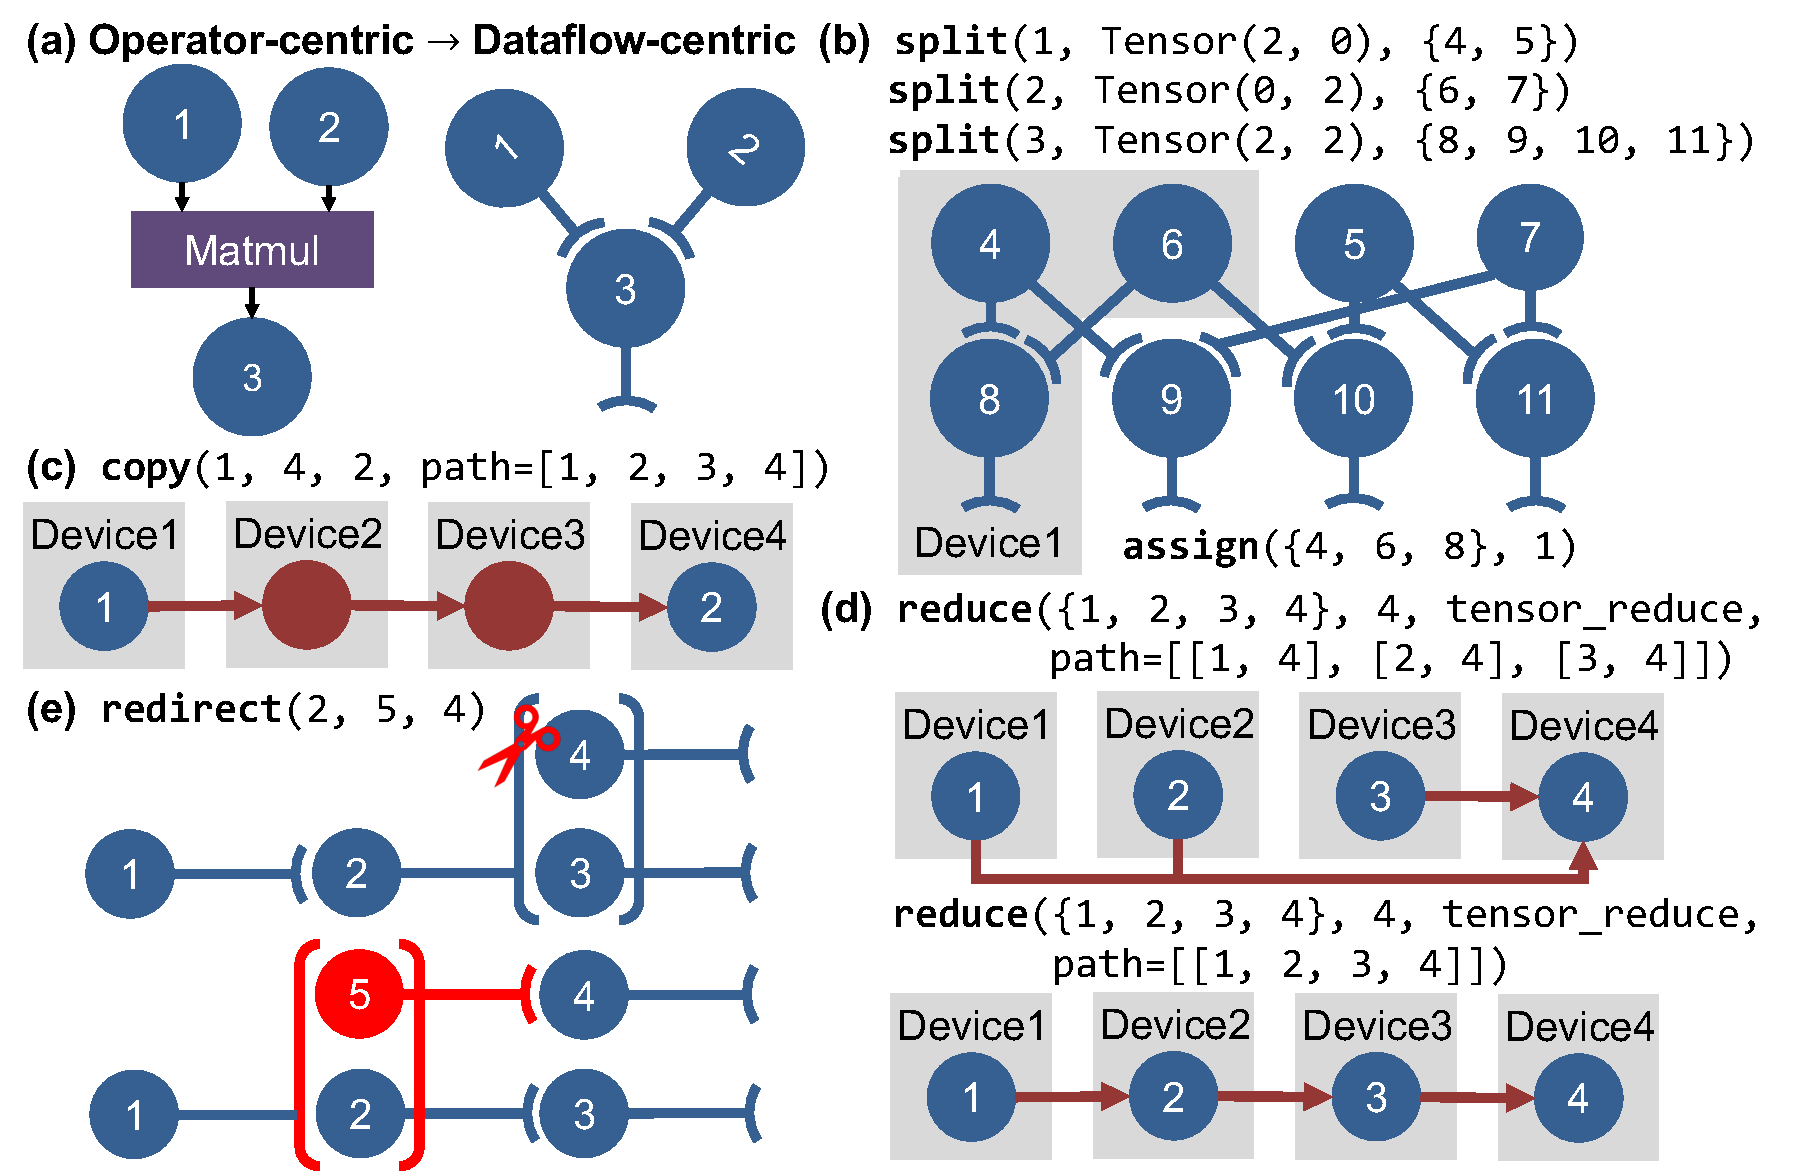
\includegraphics[width=1\linewidth]{figures/primitives.pdf}
    \caption{Illustration of dataflow-centric primitives. The \texttt{split} partitions tensors, implicitly defining operator partitioning. The \texttt{assign} primitive assigns tensors to devices, implicitly defining operator placement. The \texttt{copy}, \texttt{cut}, and \texttt{reduce} primitives manage data movement. The \texttt{redirect} primitive modifies data dependencies.}
    \label{fig:primitives}
\end{figure}

Figure \ref{fig:primitives}(a) illustrates the difference between operator-centric and dataflow-centric perspectives. From the dataflow perspective, everything in the graph is represented by the \textit{flow} of data. Each tensor is not merely a static data block in memory, but a dynamic process. The \textit{head} of the arrow in Figure \ref{fig:primitives}(a) represents the beginning of tensor generation, and the \textit{tail} represents the completion of data generation. If the flow of \texttt{tensor1} and the flow of \texttt{tensor2} meet, the generation of \texttt{tensor3} will naturally be triggered. This dataflow perspective for describing NN workloads forms the foundation of our dataflow-centric primitives.

\textbf{\texttt{split(tensor, tensor, tensors)}:} This primitive partitions a tensor into multiple sub-tensors. The first argument is the tensor to be partitioned, and the second argument is a \textit{partition vector} that specifies how to partition the first tensor. The partitioning results can be visited by the third argument. The meaning of each dimension in the \textit{partition vector} can be defined based on the specific operation. For example, for the two input tensors of a \textit{matmul} operation, the partition vector would need two dimensions, representing the number of partitions along the row and column dimensions, respectively. In FlowGen, we posit that partitioning the input data and output data implicitly partitions the computation. As illustrated in Figure \ref{fig:primitives}(b), if the operator is a \textit{matmul}, partitioning input \texttt{tensor1} along its row dimension and input \texttt{tensor2} along its column dimension naturally leads to four sub-\textit{matmul} operators. Each sub-\textit{matmul} operates on a distinct subset of the input data, resulting in four corresponding output tensors. This demonstrates that the operator partitioning can be fully and implicitly described by partitioning its input and output data.

\textbf{\texttt{assign(tensor, device)}:} This primitive assigns a tensor to a specific device. In the dataflow graph representation, a computation (operator) can begin execution only when all its required input data is available and then generate its output data.  Consequently, the mapping of a computation can be implicitly defined by mapping its input and output data. For example, as depicted in Figure \ref{fig:primitives}(b), mapping \textit{matmul} that processes the first slice of \texttt{tensor1} and the first slice of \texttt{tensor2} to \texttt{device1} can be achieved using \texttt{assign(\{tensor4, tensor6, tensor8\}, device1)}. This assigns the input tensors (\texttt{tensor4} and \texttt{tensor6}) and the output tensor (\texttt{tensor8}) of \texttt{matmul[4][6]} to \texttt{device1}, thereby implicitly mapping the associated computation.

\textbf{\texttt{copy(src\_tensor, device, dst\_tensor, path)}:} This primitive copies the tensor specified by \texttt{src\_tensor} from its current device to the target \texttt{device}. A new tensor pointer, \texttt{dst\_tensor}, is created to access the copied tensor on the destination device. \texttt{path} describes the copy path from \texttt{src\_tensor} to \texttt{dst\_tensor}. For example, as shown in Figure \ref{fig:primitives}(c), if we copy \texttt{tensor1} from device 1 to device 4, then \texttt{path} = [1, 2, 3, 4].

% \textbf{\texttt{cut(src\_tensor, device, dst\_tensor, path)}:} This primitive moves a tensor (\texttt{src\_tensor}) from its current device to the target \texttt{device}. A new tensor pointer, \texttt{dst\_tensor}, is created to access the moved tensor on \texttt{device}, and the original \texttt{src\_tensor} is freed from memory. \texttt{path} describes the movement path from \texttt{src\_tensor} to \texttt{dst\_tensor}. This is similar to \texttt{copy}, but the source tensor is deallocated.

\textbf{\texttt{reduce(src\_tensors, device, dst\_tensor, path)}:} This primitive performs a reduction operation (e.g., sum, average) across a set of tensors (\texttt{src\_tensors}). The result is stored in a new tensor pointer (\texttt{dst\_tensor}) located on the specified \texttt{device}. The \texttt{path} argument describes the reduction path of \texttt{src\_tensors} to \texttt{dst\_tensor}. For example, in Figure \ref{fig:primitives}(d), if the reduction happens on device 4, the \texttt{path} would be [[1, 4], [2, 4], [3, 4]]. If the reduction is performed sequentially, then \texttt{path} = [[1, 2, 3, 4]].

\textbf{\texttt{redirect(tensor1, tensor2, tensor3)}:} This primitive redirects data dependencies between tensors. As shown in Figure \ref{fig:primitives}(e), each tensor argument can be viewed as a flow of tensor, where the \textit{head} represents \texttt{tensor->start} (initiation of \texttt{tensor} generation, equal to triggering the corresponding computation) and the \textit{tail} represents \texttt{tensor->complete} (indicating the completion of data generation of \texttt{tensor}, equal to the computation's completion). As illustrated in Figure \ref{fig:primitives}(e), if the flow of \texttt{tensor4} initially depended on the flow of \texttt{tensor2}, the \texttt{redirect} primitive creates \texttt{tensor5}, alters the dependency to \texttt{tensor2} and copies the input dependencies of \texttt{tensor2} to \texttt{tensor5}. From a dataflow perspective, the production of \texttt{tensor4} initially depends on the completion of \texttt{tensor2}; after redirection, it depends on \texttt{tensor5}. This primitive is useful for implementing techniques such as activation recomputation, where an intermediate tensor is recomputed rather than stored, thereby saving memory (Section \ref{sec:recompute}).

\textbf{\texttt{order(tensor1, tensor2)}:} This primitive enforces a temporal ordering between two tensor-related events, which implies that \texttt{tensor1->complete} happens before \texttt{tensor2->start}. This is essential for ensuring correct execution order between different events, which can help to optimize computation, communication, and memory consumption.

% \textbf{\texttt{order(tensor1/event1, tensor2/event2)}:} This primitive enforces a temporal ordering between two events. If the arguments are tensors, it represents specific events related to those tensors (\textit{head} or \textit{tail} of a tensor flow). \texttt{order(tensor, event)} implies \texttt{tensor->complete} happens before \texttt{event}. \texttt{order(event, tensor)} implies \texttt{event} happens before \texttt{tensor->start}. \texttt{order(tensor1, tensor2)} implies \texttt{tensor1->complete} happens before \texttt{tensor2->start}. If both arguments are events, \texttt{order(event1, event2)} means \texttt{event1} happens before \texttt{event2}. This is essential for ensuring correct execution order between different events, which can help to optimize computation, communication, and memory consumption.

Leveraging these seven primitives, domain experts can construct arbitrary search spaces for parallelization plans, encompassing a wide range of DNN models and co-optimizing dataflow and computation. These search spaces are decoupled from specific model implementations, enabling a clean separation between model definition and the specification of search spaces and policies. Crucially, FlowGen's \textbf{dataflow-centric} approach, in contrast to prior operator-centric methods, facilitates the explicit co-optimization of computation and data movement. Notably, all three primitives in nnScaler can be expressed by primitives in FlowGen (\texttt{partition}, \texttt{assign}, \texttt{order}), demonstrating that the parallelization search space constructible by nnScaler is \textbf{strictly smaller} than that of FlowGen. While our primitives provide extensive flexibility, the resulting search spaces for large-scale models can be enormous, potentially involving thousands of tensors and devices and exhibiting combinatorial complexity. To address this challenge, FlowGen allows domain experts to define constraints when applying primitives. These constraints effectively prune the search space, making efficient search tractable. In the following sections, we demonstrate how these primitives and constraints can be combined to define practical, pruned search spaces, including novel strategies that are beyond the expressive capabilities of existing operator-centric frameworks (Section \ref{sec:constraints}).


\section{Constraint-Pruned Search Space}
\label{sec:new_strategies}

Like nnScaler, FlowGen employs constraints as parameterized arguments to the primitives listed in Table \ref{tab:primitives}. Specifying concrete values for all arguments effectively reduces the search space to a single, deterministic parallelization plan. This section illustrates the construction of a wide variety of parallelization plans using FlowGen's primitives and constraints.  We structure the discussion as follows: Section \ref{sec:operator_constraints} demonstrates how FlowGen's dataflow-centric primitives can express any search space constructible using nnScaler's operator-centric primitives. Section \ref{sec:dataflow_constraints} highlights FlowGen's unique capability to represent dataflow optimizations and the co-optimization of dataflow and computation, which are beyond the reach of prior approaches. Finally, Section \ref{sec:new_constraints} explores FlowGen's applicability to emerging workloads, showcasing its potential for discovering novel optimization opportunities.


\subsection{Constraints for Operator-Centric Search Spaces}
\label{sec:operator_constraints}

\subsubsection{Data and Tensor Parallelism.} 

Table \ref{tab:dp_tp} shows the primitive program and the associated constraints for a fully-connected layer's hybrid TP and DP search space. In this example, the partition vectors \texttt{vi}, \texttt{vw}, and \texttt{vo} are searchable. Each partition vector has a dimension of 3. For \texttt{vi}, the first dimension represents the batch dimension, and the second represents the input dimension. For \texttt{vw}, the first dimension is the input dimension, and the second is the output dimension. For \texttt{vo}, the first dimension is the batch dimension, and the second is the output dimension. The last dimension of all partition vectors is the replication dimension. The constraints limit the feasible search space of these partition vectors. $D$ represents the total set of devices. The \texttt{assign} primitives map the partitioned input/output tensor groups to the devices in $D$. This example demonstrates a hybrid DP and TP strategy. For pure DP, only the first dimension of \texttt{vi} and \texttt{vo} can be non-zero (zero means no partitioning).

\begin{table}[h]
\centering
\footnotesize
\begin{tabular}{l|l}
\textbf{Primitive program} & \textbf{Constraints} \\
\hline
\texttt{vi = }input partition vector & $\mathrm{dim}(v^i) = 3$ \\ 
\texttt{vw = }weight partition vector & $\mathrm{dim}(v^w) = 3$ \\
\texttt{vo = }output partition vector & $\mathrm{dim}(v^o) = 3$ \\
\hline
\texttt{split(input, vi, split\_inputs)} & $v^i_0 = v^o_0, v^o_1 = v^w_0, v^i_2 = v^w_1$ \\
\texttt{split(weight, vw, split\_weights)} & $v^w_1 = w^o_1, v^w_2 = v^i_0$ \\
\texttt{split(output, vo, split\_outputs)} & $v^o_2 = v^i_1, v^o_0v^o_1v^i_1 = |D|$ \\
\hline
\texttt{assign(split\_inputs[i][k][j], D[i][j][k])} & \\
\texttt{assign(split\_weights[k][j][i], D[i][j][k])} & \\
\texttt{assign(split\_outputs[i][j][k], D[i][j][k])} & $(i, j, k) \neq (l, m, n)$ \\
\texttt{assign(split\_inputs[l][n][m], D[l][m][n])} & $D_{ijk}, D_{lmn} \in D$ \\
\texttt{assign(split\_weights[m][n][l], D[l][m][n])} & \\
\texttt{assign(split\_outputs[l][m][n], D[l][m][n])} & \\
\hline
\end{tabular}
\caption{Primitive program and constraints for DP and TP of a fully-connected layer}
\label{tab:dp_tp}
\end{table}

\subsubsection{Pipeline Parallelism}

PP divides a model into stages, enabling concurrent execution in a pipelined manner. FlowGen divides all tensors of a model into distinct groups $G_i$ ($0 \leq i < |D|$), where $i$ represents the $i$-th pipeline stage. These tensor groups are then assigned to different devices, as shown in Table \ref{tab:pp}. To minimize pipeline bubbles, PP divides a batch of samples into micro-batches. The input, activation, and gradient data of each stage are split along the batch dimension. These are denoted as \texttt{fMA[i][j]} and \texttt{bMA[i][j]} for the forward and backward passes of the $j$-th micro-batch in the $i$-th stage, respectively. Different micro-batches share the same weights, denoted as \texttt{W[i]} in the $i$-th stage. The constraints required to implement the 1F1B\cite{huang2019gpipe} schedule are summarized in Table \ref{tab:1f1b}, where $N$ is the number of micro-batches.

\begin{table}[h]
\centering
\footnotesize
\begin{tabular}{l|l}
\textbf{Primitive program} & \textbf{Constraints} \\
\hline
\texttt{assign(G[i], D[i])} & $i \neq j$ \\
\texttt{assign(G[j], D[j])} & $D_i, D_j \in D$ \\
\hline
\end{tabular}
\caption{Primitive program and constraints for PP.}
\label{tab:pp}
\end{table}

\begin{table}[h]
\centering
\footnotesize
\begin{tabular}{l|l}
\textbf{Primitive program} & \textbf{Constraints} \\
\hline
\texttt{A[i] = }inputs, activations, gradient in \texttt{G[i]} & \\
\texttt{W[i] = }weights in \texttt{G[i]} & \\
\texttt{v = }input, activation, gradient partition vector & \\
\hline
\texttt{split(A[i], v, MA[i][j])} & $v_0 = N, v_1, ... = 0, 0 \leq j < N $ \\
\texttt{assign(MA[i][j], D[i])} & \multirow{2}{*}{$D_i \in D$} \\
\texttt{assign(W[i], D[i])} & \\
\hline
\texttt{order(fMA[i][j], fMA[i][j+1])} & \multirow{2}{*}{$j \geq 0$} \\ 
\texttt{order(bMA[i][j], bMA[i][j+1])} &   \\
\hline
\texttt{order(fMA[i][j+ofst], bMA[i][j])} &  $\mathrm{ofst} = |D| - i - 1$ \\
\texttt{order(bMA[i][j], fMA[i][j+ofst+1])} &  $j \geq 0$ \\
\hline
\end{tabular}
\caption{Primitive program and constraints for 1F1B schedule.}
\label{tab:1f1b}
\end{table}

Combining TP and PP results in a search space known as staged SPMD (\texttt{staged\_spmd(tensors, devices)}). In this configuration, TP is applied within each stage of PP. This is accomplished by replacing the single device specified in the PP constraints (Table \ref{tab:pp}) with a set of devices for each stage. Subsequently, the TP constraints (Table \ref{tab:dp_tp}) are applied within each of these device sets. We omit the detailed expansion for brevity.

\subsubsection{Streamlined Split Operators}
\label{sec:streamline}

Traditionally, in TP, each partition is assigned to a dedicated device. nnScaler\cite{lin2024nnscaler} introduces an optimization where multiple partitions can share a single device, with computations executed in a streamlined manner. Consider a scenario where different partitioned output data require a reduction. While this streamlined execution might decrease computation speed, the reduced communication overhead due to fewer devices can potentially lower the overall cost and improve performance. Let $D$ represent the set of devices. We can increase the number of TP partitions to $C \cdot |D|$ and assign $C$ corresponding input and output data partitions to a single device. For brevity and w.l.o.g., we consider pointwise operators, where the input and output tensors have identical shapes and partitioning schemes. The constraints are detailed in Table \ref{tab:streamline}, where $C$ represents a searchable parameter.

\begin{table}[h]
\centering
\footnotesize
\begin{tabular}{l|l}
\textbf{Primitive program} & \textbf{Constraints} \\
\hline
\texttt{v = }partition vector & \\
\hline
\texttt{split(input, v, split\_inputs)} & \multirow{2}{*}{$\mathrm{prod}(v) = C \cdot |D|$} \\
\texttt{split(output, v, split\_outputs)} &  \\
\hline
\texttt{assign(split\_inputs[i][j], D[i])} &  $0 \leq j < C$ \\
\texttt{assign(split\_outputs[i][j], D[i])} &  $D_i \in D$ \\
\hline
\end{tabular}
\caption{Primitive program and constraints for streamlined split operators where each device have multiple TP partitions.}
\label{tab:streamline}
\end{table}

Suppose we need to perform a reduction across the tensors within \texttt{split\_outputs}. Intuitively, we should first reduce the tensors within each device and then reduce the per-device results to obtain the final result. However, this kind of hierarchical reduction behavior cannot be formally defined in nnScaler's operator-centric representation. This very simple example demonstrates a core limitation of nnScaler's operator-centric representation. For the worst case, after each split operator's computation, a cross-device reduction could be performed instead of an intra-device reduction. Such a dataflow organization would negate the intended benefit of reduced communication overhead. We will show how FlowGen's primitives tackle this problem in Section \ref{sec:hierarchical_reduce}.


\subsubsection{Staged SPMD with Large Embedding Table}

For transformer models, particularly multi-lingual models\cite{raffel2020exploring}, the embedding table (denoted as $E$) occupies substantial memory but demands minimal computation. Traditional PP would prioritize assigning devices to accommodate $E$, allocating the remaining devices to other operators. This approach, however, leads to imbalanced hardware utilization. nnScaler introduced an optimization that distributes the embedding table across all devices. Consequently, other operators can share resources, deviating from the conventional assumption that operators in different pipeline stages are confined to distinct sets of devices. Table \ref{tab:embedding} illustrates this optimization.

\begin{table}[h]
\centering
\footnotesize
\begin{tabular}{l|l}
\textbf{Primitive program} & \textbf{Constraints} \\
\hline
% \texttt{vi = }input partition vector & $\mathrm{dim}(v^i) = 2$ \\
\texttt{ve = }embedding table partition vector & $\mathrm{dim}(v^i) = 2$ \\
% \texttt{vo = }output partition vector & $\mathrm{dim}(v^i) = 2$ \\
\texttt{tensors = }other tensors excluding embedding& \\
\hline
\texttt{split(embedding\_table, ve, split\_embedding\_tables)} & $v^e_0 v^e_1 = |D|$ \\
\texttt{assign(split\_embedding\_tables[i], D[i])} & $D_i \in D$ \\
\hline
\texttt{staged\_spmd(tensors, D)} & \\
\hline
\end{tabular}
\caption{Primitive program and constraints for distributing the embedding table across devices and device sharing across different pipeline stages.}
\label{tab:embedding}
\end{table}

\subsubsection{3F1B for AlphaFold2}

In AlphaFold2\cite{jumper2021highly}, training each micro-batch necessitates three forward passes and one backward pass, a pattern not supported by the standard 1F1B schedule. A naive sequential execution of micro-batches would introduce pipeline bubbles and accumulate numerous unnecessary intermediate activations, resulting in inefficiency. To mitigate this, nnScaler employs a 3F1B schedule, which interleaves the forward and backward passes of different micro-batches while adhering to temporal order constraints. In Table \ref{tab:3f1b}, \texttt{fpMA[i][j]} denotes the tensor groups of the $j$-th micro-batch in the $p$-th forward pass at pipeline stage $i$. The term $\mathrm{ofst}$ is defined as $S - i - 1$, where $S$ represents the total number of pipeline stages, and $N$ represents the number of micro-batches. Table \ref{tab:3f1b} details the constraints associated with the 3F1B schedule.

\begin{table}[h]
  \centering
  \footnotesize
  \begin{tabular}{l|l}
  \textbf{Primitive program} & \textbf{Constraints} \\
  \hline
  \texttt{A[i] = }inputs, activations, gradient in \texttt{G[i]} & \\
  \texttt{W[i] = }weights in \texttt{G[i]} & \\
  \texttt{v = }input, activation, gradient partition vector & \\
  \hline
  \texttt{split(A[i], v, MA[i][j])} & $v_0 = N, v_1, ... = 0, 0 \leq j < N $ \\
  \texttt{assign(MA[i][j], D[i])} & \multirow{2}{*}{$D_i \in D$} \\
  \texttt{assign(W[i], D[i])} & \\
  \hline
  \texttt{order(f1MA[i][j+1], f2MA[i][j])} & $j \geq 0$ \\ 
  \texttt{order(f2MA[i][k+1], f2MA[i][k])} &  $k \geq 0$ \\
  \texttt{order(f3MA[i][l+ofst], bMA[i][l])} &  $l \geq 0$ \\
  \hline
  \end{tabular}
  \caption{Primitive program and constraints for 3F1B schedule.}
  \label{tab:3f1b}
\end{table}

\subsection{Constraints for Dataflow-Centric Search Spaces}
\label{sec:dataflow_constraints}

In this section, we showcase multiple prevalent dataflow optimizations and dataflow-compute co-optimizations, which, despite their popularity and significant impact on computational time, communication overhead, memory consumption, and overall performance in large-scale NN training systems, cannot be expressed by any existing frameworks. This discrepancy underscores the potential of FlowGen to unlock substantial optimization spaces, thereby assisting domain experts in exploiting the full performance capabilities of existing training systems.

\subsubsection{Cross-Mesh Resharding}

Cross-mesh resharding arises from different TP strategies employed across various stages in staged SPMD. This necessitates aligning the output data layout of one stage with the input data layout of the subsequent stage. The efficiency of cross-mesh resharding may significantly impact communication costs between device meshes. Because inter-mesh communication bandwidth is typically lower than intra-mesh bandwidth, inefficient resharding strategies can become a performance bottleneck. However, planning for cross-mesh resharding requires dataflow management, a capability not expressible by existing tools. We demonstrate how FlowGen can be used to implement different cross-mesh resharding strategies.

\begin{figure}[h]
  \centering
  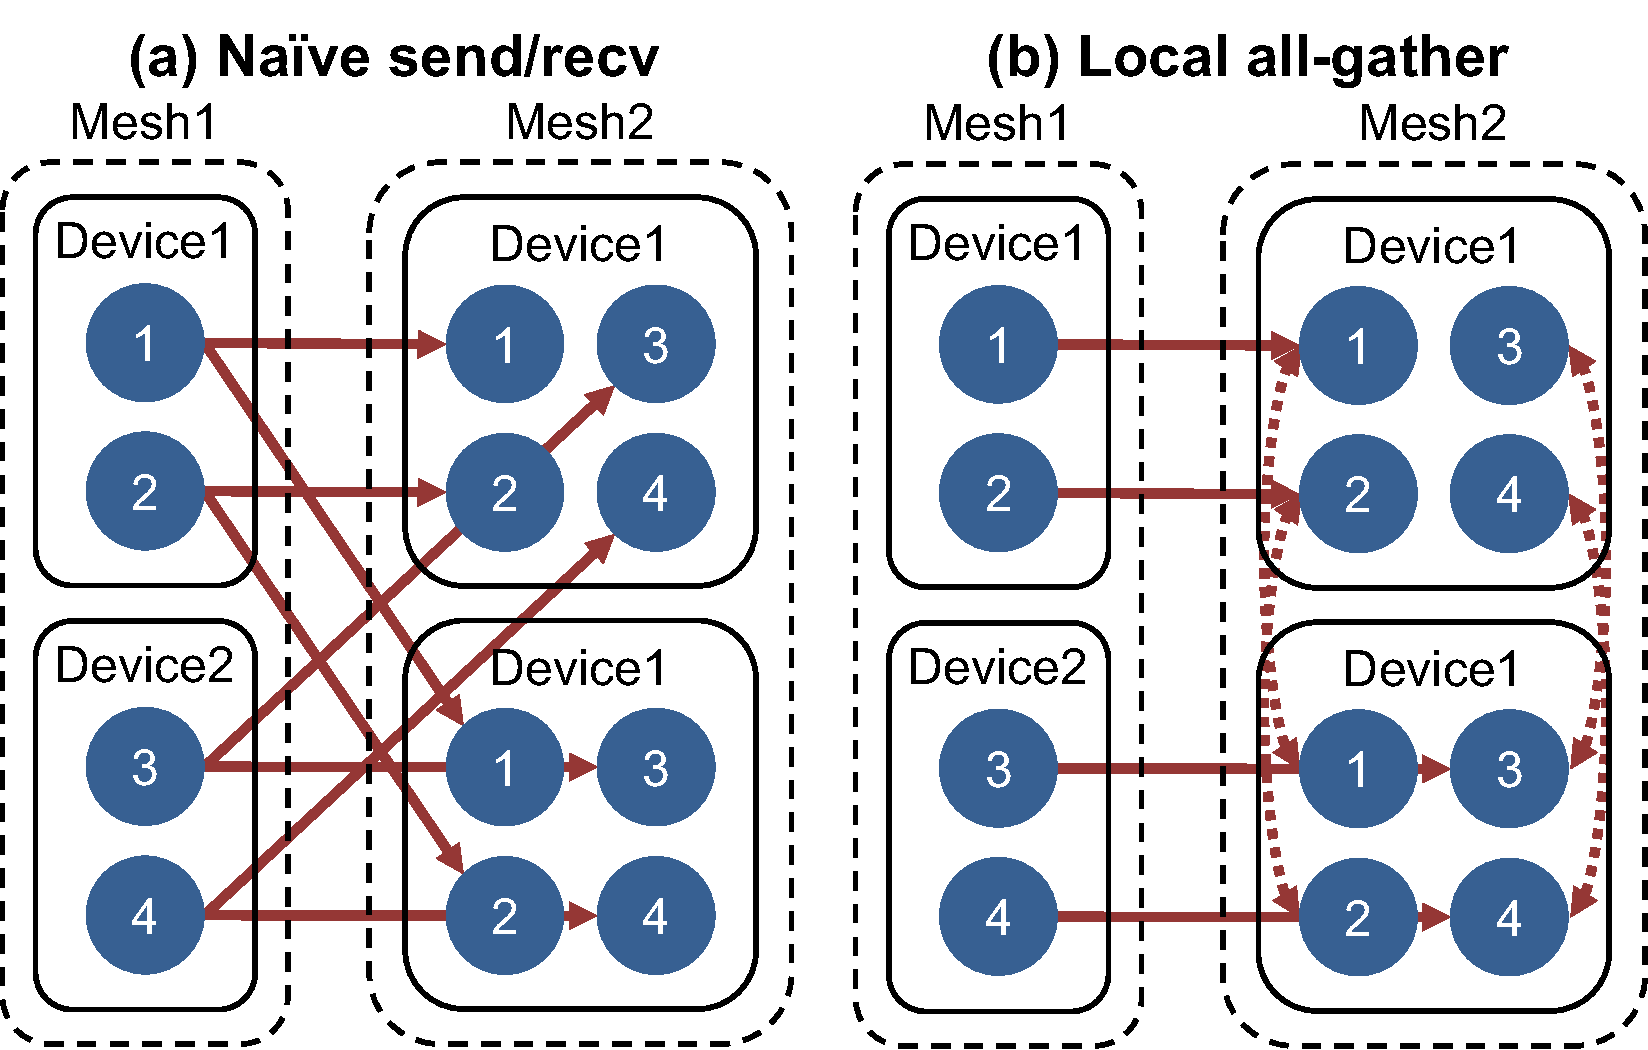
\includegraphics[width=1\linewidth]{figures/cross_mesh.pdf}
  \caption{Cross-mesh resharding strategies between consecutive pipeline stages. (a) Naive implementation using peer-to-peer (P2P) send/receive operations between Mesh1 and Mesh2. (b) Optimized Alpa implementation: Tensors 1-4 are first transferred between meshes via send/recv, followed by intra-mesh all-gather operations on Mesh2. Solid arrows represent cross-mesh communication, while dashed arrows indicate intra-mesh operations.}
  \label{fig:cross_mesh}
\end{figure}

Figure \ref{fig:cross_mesh} illustrates two cross-mesh resharding strategies. For Figure \ref{fig:cross_mesh}(a), the primitive program and constraints are shown in Table \ref{tab:cross_mesh_p2p}, where \texttt{copy(tensor, D)} is a composite primitive, equivalent to a series of primitives: \texttt{copy(tensor, D[0])}, \texttt{copy(tensor, D[1])}, ... This implementation can lead to redundant send/receive operations.

\begin{table}[h]
\centering
\footnotesize
\begin{tabular}{l|l}
\textbf{Primitive program} & \textbf{Constraints} \\
\hline
\texttt{copy(T[i], D, -, path)} & $T_i \in T$ \\
\hline
\end{tabular}
\caption{Primitive program and constraints for cross-mesh resharding: naive P2P send/recv.}
\label{tab:cross_mesh_p2p}
\end{table}

For the local all-gather optimization in Figure \ref{fig:cross_mesh}(b), the primitive program and constraints are shown in Table \ref{tab:cross_mesh_local}, where the tensors on Mesh1 are first copied to Mesh2 without redundancy, followed by an intra-mesh all-gather operation on Mesh2. This reduces slow cross-mesh communication.

\begin{table}[h]
\centering
\footnotesize
\begin{tabular}{l|l}
\textbf{Primitive program} & \textbf{Constraints} \\
\hline
\texttt{copy(T[i], D[j], T'[i], path)} & $\forall T_i \in T, D_j \in D$ \\
\hline
\texttt{copy(T'[i], D\textbackslash D[j], -, path)} & $\mathrm{Set}(\mathrm{path}) = \{i|D_i \in D\backslash D_j\}$ \\
\hline
\end{tabular}
\caption{Primitive program and constraints for cross-mesh resharding: local all-gather.}
\label{tab:cross_mesh_local}
\end{table}

As shown in Table \ref{tab:cross_mesh_local}, the first step, cross-mesh copy, can copy the tensor from Mesh1 to any device in Mesh2. However, copying from Mesh1-Device1 to Mesh2-Device1 might be the best choice (closest physical distance, fastest transfer speed). To achieve this optimization, we can further constrain the device index to which the cross-mesh copy is performed, as shown in Table \ref{tab:cross_mesh_local_align}, which will lead to the dataflow pattern in Figure \ref{fig:cross_mesh}(b). Furthermore, we can also constrain the intra-mesh broadcast path. The second constraint in Table \ref{tab:cross_mesh_local_align} implies that starting from device $j$, data is transferred to device $j + kN$ at each step $k$, where $N$ can be a searchable parameter.

\begin{table}[h]
  \centering
  \footnotesize
  \begin{tabular}{l|l}
  \textbf{Primitive program} & \textbf{Constraints} \\
  \hline
  \texttt{copy(T[i], D[j], T'[i], path)} & $\forall T_i \in T, D_j \in D, j = i \mathbin{/\mkern-3mu/} |D|$ \\
  \hline
  \multirow{3}{*}{\texttt{copy(T'[i], D\textbackslash D[j], -, path)}} & $\mathrm{Set}(\mathrm{path}) = \{i|D_i \in D \backslash D_j\}$ \\
   & $\mathrm{path}[0] = j, \forall k \geq 0:$ \\
   & $\mathrm{path}[k + 1] = (\mathrm{path}[k] + N) \, \mathrm{mod} \, |D|$ \\
  \hline
  \end{tabular}
  \caption{Primitive program and constraints for cross-mesh resharding: local all-gather with better locality and constrained broadcast path.}
  \label{tab:cross_mesh_local_align}
  \end{table}

\subsubsection{Parameter Server}

In the parameter server architecture, several key decisions must be made: identifying the devices that will act as parameter servers, defining the method for aggregating gradients to these servers, and establishing how updated parameters are distributed from the servers back to the compute devices. Figure \ref{fig:ps_hr} illustrates two distinct implementations of this architecture. The first approach designates one of the compute devices as the server; parameters are then passed sequentially to all other devices. The second approach utilizes a dedicated, separate device as the parameter server. In this configuration, all compute devices and the parameter server employ independent communication paths for gradient aggregation and parameter broadcasting. Tables \ref{tab:parameter_server1} and \ref{tab:parameter_server2} detail the primitive programs and associated constraints for each of these implementations, respectively.

\begin{figure}[h]
    \centering
    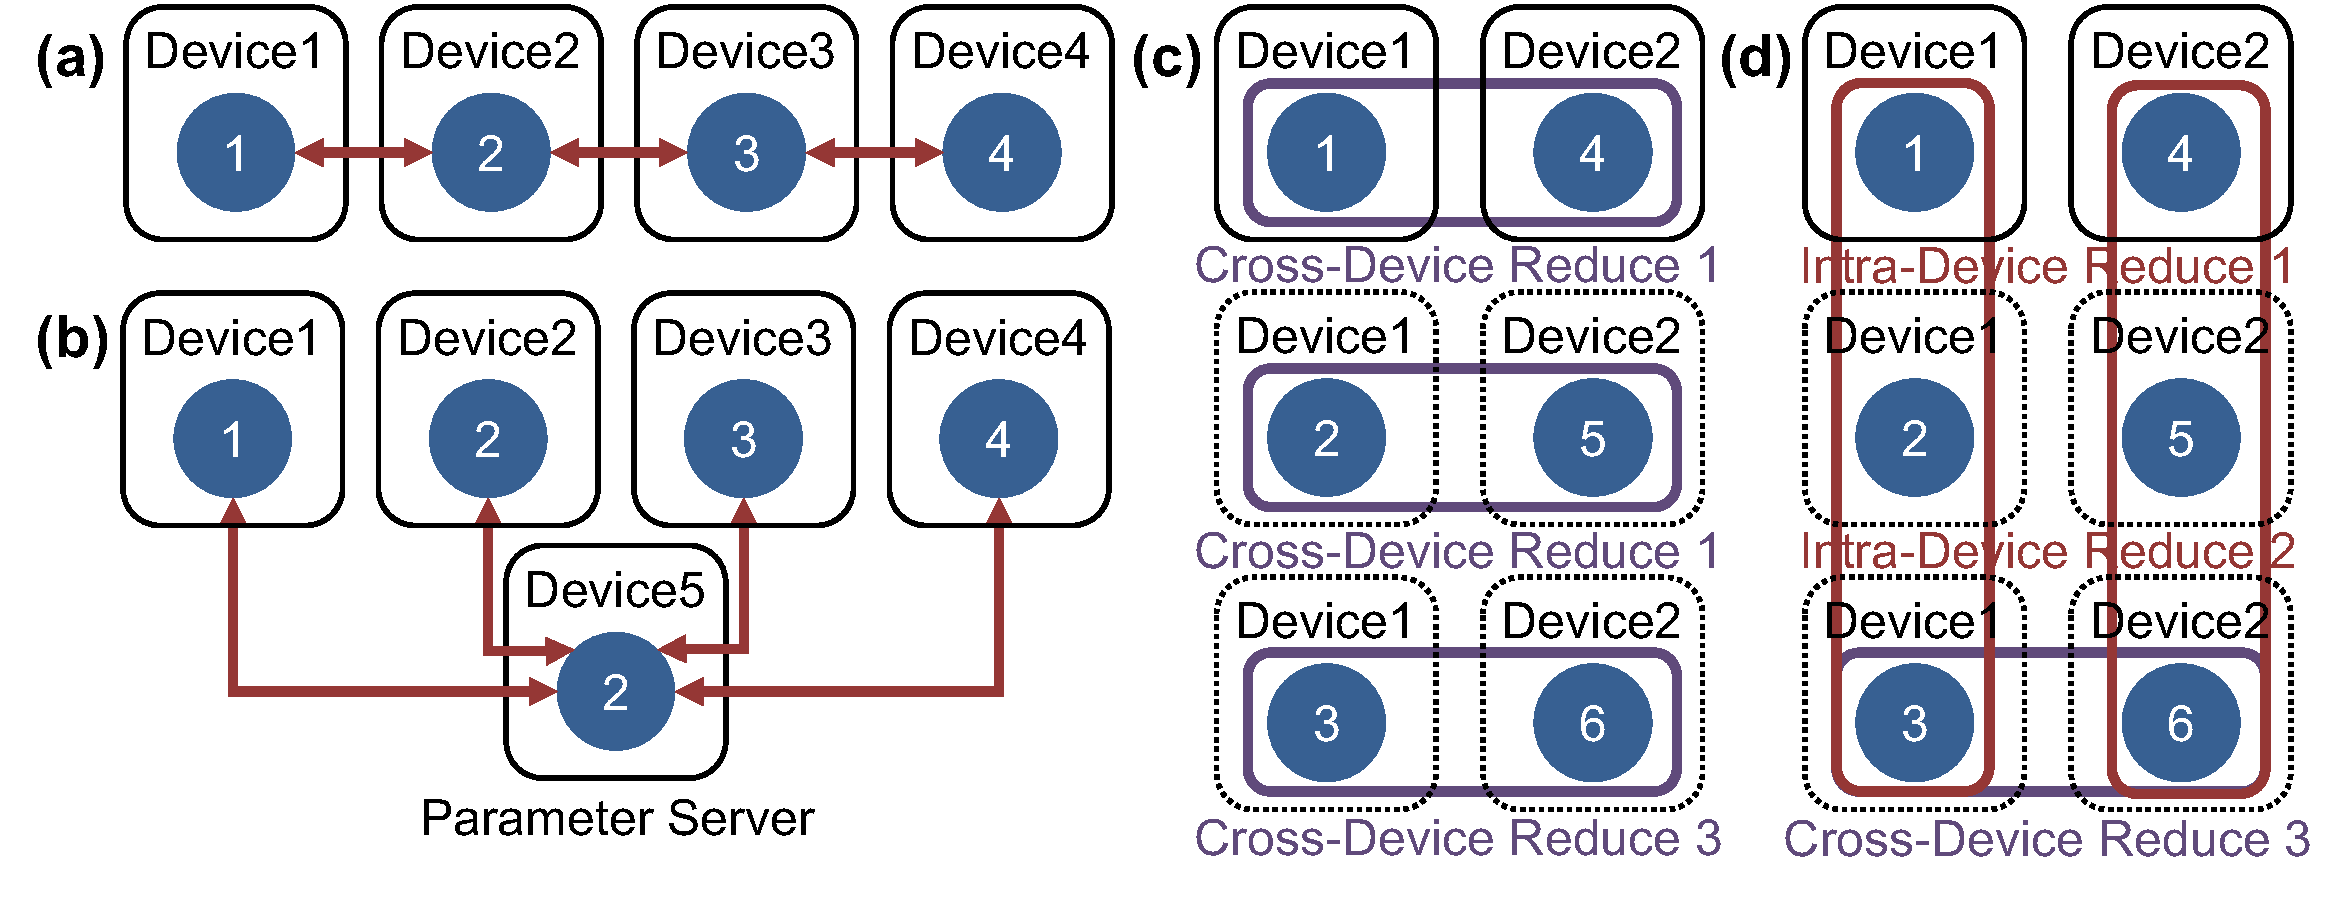
\includegraphics[width=1\linewidth]{figures/parameter_server_hierarchical_reduce.pdf}
    \caption{(a-b) Two implementations of the parameter server architecture. (c-d) Two implementations of hierarchical reduce.}
    \label{fig:ps_hr}
\end{figure}


\begin{table}[h]
\centering
\footnotesize
\begin{tabular}{l|l}
\textbf{Primitive program} & \textbf{Constraints} \\
\hline
\texttt{W = }updated parameters & \\
\hline
\texttt{reduce(G, D[i])} & $D_i \in D$ \\
\hline
\texttt{copy(W, D\textbackslash D[i])} &  \\
\hline
\end{tabular}
\caption{Primitive program and constraints for parameter server (parameter server can also be a computing device).}
\label{tab:parameter_server1}
\end{table}

\begin{table}[h]
  \centering
  \footnotesize
  \begin{tabular}{l|l}
  \textbf{Primitive program} & \textbf{Constraints} \\
  \hline
  \texttt{W = }updated parameters & \\
  \texttt{PS = }parameter server & \\
  \hline
  \texttt{reduce(G, PS)} & \\
  \hline
  \texttt{copy(W, D)} & $\mathrm{PS} \notin D$ \\
  \hline
  \end{tabular}
  \caption{Primitive program and constraints for parameter server (independent parameter server).}
  \label{tab:parameter_server2}
  \end{table}


\subsubsection{Streamlined Split Operators with Hierarchical Reduce}
\label{sec:hierarchical_reduce}

% 在Section \ref{sec:streamline}里面，我们提到了一个问题，即nnScaler的本意是通过让多个split operator来以streamline的方式执行，从而降低整体的memory consumption和communication cost. However，only by nnScaler's representations, the dataflow behaviors are undefined, 错误的dataflow plan可能会导致无法起到本来的优化效果。我们在Figure \ref{fig:hierarchical_reduce}中展示了这一点

We illustrate how FlowGen addresses the limitation of nnScaler's representation for streamlined split operators with hierarchical reduce in Figure \ref{fig:ps_hr}. Table \ref{tab:reduce_bad} and Table \ref{tab:reduce_good} demonstrate two ways to describe hierarchical reduce using FlowGen. Here, \texttt{T[i][j]} represents the j-th tensor on the i-th device, \texttt{T[:][j]} represents the j-th tensor across all devices, and \texttt{T[i][:]} represents all tensors on the i-th device. The first is a bad case, where each device performs a cross-device reduce after completing a split operator's computation. The final result is obtained by another cross-device communication among all reduction results. Overall, this requires $C$ cross-device reduce operations. The second is a good implementation, where we perform reduction on the current device after each split operator. Consequently, we only need one final cross-device reduce. Although this optimization is straightforward, nnScaler's operator-centric primitives cannot accurately define this behavior, which can lead to missed optimization opportunities in more complex scenarios. FlowGen's \texttt{reduce} primitive explicitly defines the reduction behavior, ensuring the intended communication optimization.

\begin{table}[h]
\centering
\footnotesize
\begin{tabular}{l|l}
\textbf{Primitive program} & \textbf{Constraints} \\
\hline
\texttt{T[i][:] = }tensors on \texttt{D[i]} & \\
\hline
\texttt{reduce(T[:][j], D[i], T'[j])} & $D_i \in D, T_j' \in T'$ \\
\texttt{reduce(T', D[k])} & $D_k \in D$ \\
\hline
\end{tabular}
\caption{Primitive program and constraints for hierarchical reduce (bad case).}
\label{tab:reduce_bad}
\end{table}

\begin{table}[h]
\centering
\footnotesize
\begin{tabular}{l|l}
\textbf{Primitive program} & \textbf{Constraints} \\
\hline
\texttt{T[i][:] = }tensors on \texttt{D[i]} & \\
\hline
\texttt{reduce(T[i][:], D[i], T'[i])} & $D_i \in D, T_i' \in T'$ \\
\texttt{reduce(T', D[j])} & $D_j \in D$ \\
\hline
\end{tabular}
\caption{Primitive program and constraints for hierarchical reduce (good case).}
\label{tab:reduce_good}
\end{table}


\subsubsection{Offloading}

Offloading is a technique that moves data to other devices (e.g., from GPU device to CPU host) to reduce the memory pressure on the original device, as illustrated in Figure \ref{fig:offloading}. It requires the cooperation between computation and data movement strategy. Table \ref{tab:offloading} shows an example of representing offloading primitives in FlowGen. In the training of LLMs, activations generated during the forward pass (like \texttt{f1}) need to be used in the backward pass, consuming significant device memory. Offloading addresses this by moving such activations to host memory. As shown in Table \ref{tab:offloading}, the first primitive represents the operation to offload activation \texttt{f1} to the host. The first constraint specifies that this offload must occur after the forward computation \texttt{f2}. Subsequently, the activation needs to be prefetched back to the device memory before it is required by the backward pass computation \texttt{b1}. This prefetch operation is represented by the second primitive. The ordering constraints ensure that the prefetch happens after the offload and before the backward computation \texttt{b1}. FlowGen enables searching for the optimal timing for both the offload (\texttt{event1}) and prefetch (\texttt{event2}) operations, respecting these dependencies, to effectively manage memory and minimize performance impact.

\begin{figure}[h]
  \centering
  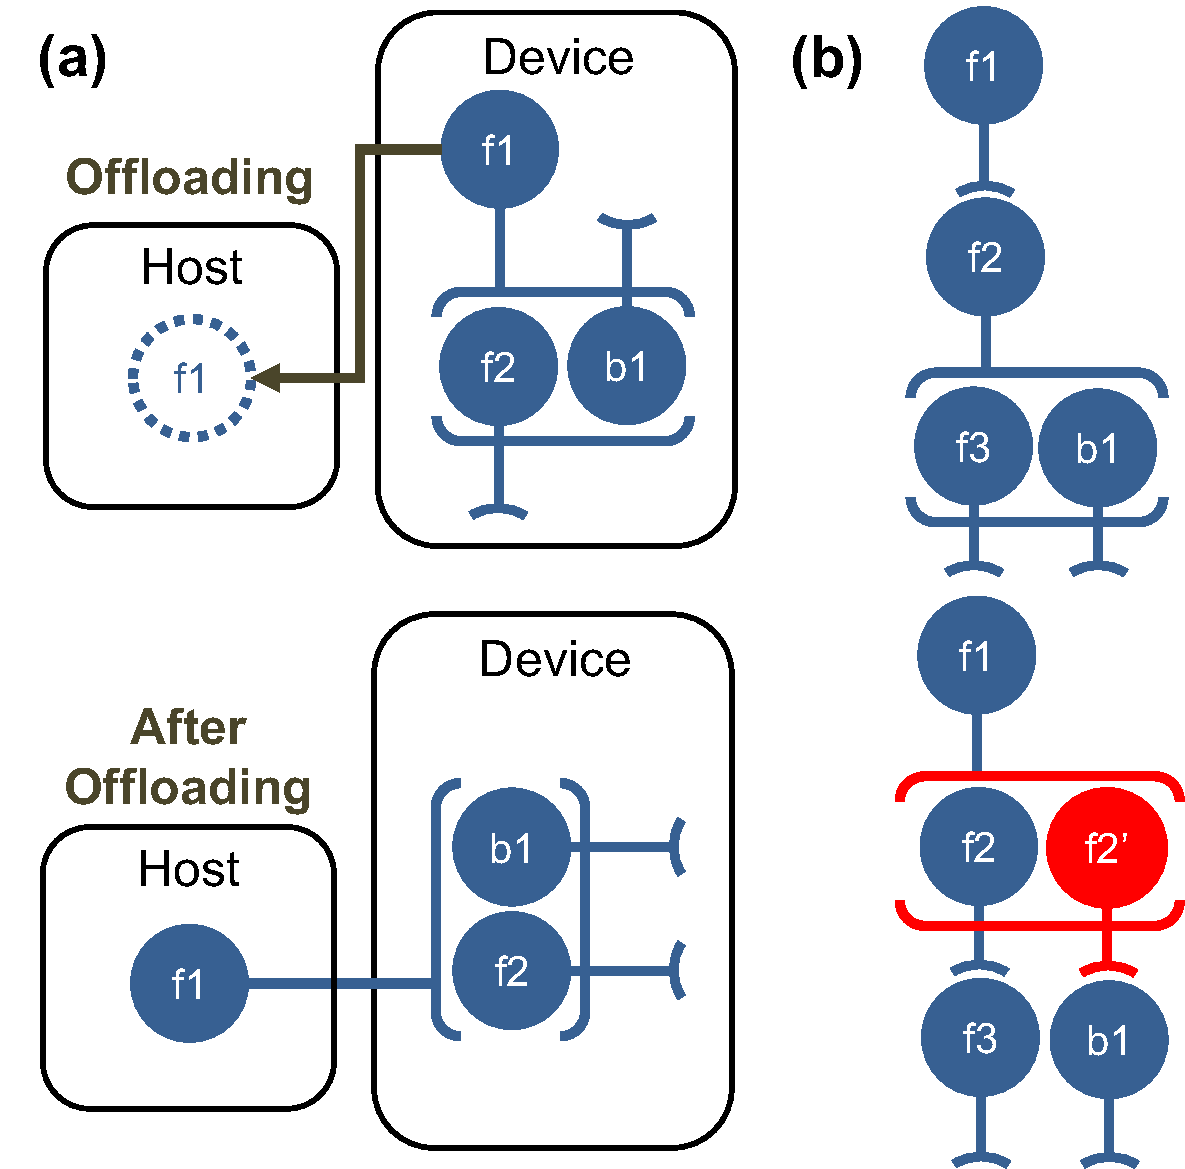
\includegraphics[width=1\linewidth]{figures/offload_recompute.pdf}
  \caption{(a-b) Illustration of offloading. Activations computed on the device are moved to host memory to free up device memory, and later prefetched back to the device when needed for the backward pass.}
  \label{fig:offloading}
\end{figure}

\begin{table}[h]
  \centering
  \footnotesize
  \begin{tabular}{l|l}
  \textbf{Primitive program} & \textbf{Constraints} \\
  \hline
  % \texttt{redirect(f1, f1', {f2, b1})}
  \texttt{f1' = copy(f1, host, path)} & \texttt{order(f2, f1')} \\
  \hline
  \multirow{2}{*}{\texttt{f1'' = copy(f1', device, path)}} & \texttt{order(f1', f1'')} \\
   & \texttt{order(f1'', b1)}  \\
  \hline
  \end{tabular}
  \caption{Primitive program and constraints for offloading.}
  \label{tab:offloading}
\end{table}


\subsubsection{Recomputation}
\label{sec:recompute}

Recomputation is a memory-saving technique where activations computed during the forward pass are freed and then recomputed later during the backward pass when needed. This avoids storing all intermediate activations, checkpointing only a select few. Figure \ref{fig:offloading} illustrates an example scenario involving recomputation. Table \ref{tab:recompute} shows the corresponding primitive program representation in FlowGen. First, a \texttt{redirect} primitive modifies data dependencies. For example, assume a backward operation \texttt{b2} initially depends on activation \texttt{f2}. Using \texttt{redirect(f2, f2', b2)}, we change this dependency to a placeholder tensor \texttt{f2'}, meaning \texttt{b2} no longer directly requires the original \texttt{f2}. Our runtime system (detailed in Section \ref{sec:compiler}) manages memory automatically via reference counting, freeing memory when a tensor's reference count reaches zero. After the redirection, if no other operation requires \texttt{f2} (e.g., after the generation of \texttt{f3} completes), its memory can be released. However, since the recomputation placeholder \texttt{f2'} depends on \texttt{f1}, \texttt{f1}'s reference count remains non-zero, effectively checkpointing \texttt{f1}. As shown in the table, the constraint ensure this recomputation happens after \texttt{f3} and before \texttt{b2}. FlowGen can search for the optimal point to perform this recomputation.

\begin{table}[h]
  \centering
  \footnotesize
  \begin{tabular}{l|l}
  \textbf{Primitive program} & \textbf{Constraints} \\
  \hline
  \texttt{redirect(f2, f2', b2)} & \texttt{order(f3, f2')} \\
  \hline
  \end{tabular}
  \caption{Primitive program and constraints for recomputation.}
  \label{tab:recompute}
\end{table}

\subsubsection{FSDP}

FSDP is a widely-adopted optimization technique that requires careful coordination between computation and data movement. In FSDP, model parameters are sharded across devices to reduce per-device memory consumption. During training, each device only holds a portion of the parameters. When a layer needs to perform computation, the required parameters are gathered from other devices, used for computation, and then immediately freed to save memory. The gradients follow a similar pattern - they are computed locally, synchronized across devices, and then immediately sharded again. This intricate interplay between parameter/gradient movement and computation cannot be expressed using existing operator-centric frameworks\cite{lin2024nnscaler}. Table \ref{tab:fsdp} shows how FlowGen's primitives can naturally represent this coordination.

\begin{table}[h]
\centering
\footnotesize
\begin{tabular}{l|l}
\textbf{Primitive program} & \textbf{Constraints} \\
\hline
\texttt{split(input, vi, split\_inputs[:])} & $v^i_0 = |D|, v^i_1, ... = 0$ \\
\texttt{assign(split\_inputs[i], D[i])} & $D_i \in D$ \\
\texttt{split(weight, vw, split\_weights[:])} & $\prod_i v^w_i = |D|$ \\
\texttt{assign(split\_weights[i], D[i])} & $D_i \in D$ \\
\texttt{split(output, vo, split\_outputs[:])} & $v^o = v^i$ \\
\texttt{assign(split\_outputs[i], D[i])} & $D_i \in D$ \\
\texttt{split(gradient, vg, split\_gradients[:][:])} & $v^g_0 = v^i_0, v^g[1:] = v^w[1:]$\\
\texttt{assign(split\_gradients[i][:], D[i])} & $D_i \in D$ \\
\texttt{split(opt\_state, vs, split\_opt\_states)} & $v^s = v^w$ \\
\texttt{assign(split\_opt\_states[i], D[i])} & $D_i \in D$ \\
\hline
\texttt{fweights[i] = copy(split\_weights[:], D[i])} & \multirow{5}{*}{$i \in \{0, 1, ..., |D| - 1\}$} \\
\texttt{order(fweights[i], split\_outputs[i])} &  \\
\texttt{bweights[i] = copy(split\_weights, D[i])} &  \\
\texttt{order(bweights[i], split\_gradients[i])} & \\
\texttt{reduce(split\_gradients[:][i], D[i])} & \\
\hline
\multicolumn{2}{l}{input partition vector $v^i$, parameter partition vector $v^w$} \\
\multicolumn{2}{l}{output partition vector $v^o$, gradient partition vector $v^g$} \\
\multicolumn{2}{l}{optimizer state partition vector, $v^s$} \\
\hline
\end{tabular}
\caption{Primitive program and constraints for FSDP.}
\label{tab:fsdp}
\end{table}

\subsubsection{Memory Balance Scheduling in 1F1B}


\subsection{Constraints for Emerging Workloads}
\label{sec:new_constraints}

\subsubsection{Fine-Grained FSDP \& PSDP}

\subsubsection{DeepSeek-MoE}

\subsubsection{GRPO}


\section{Dataflow-Centric Plan Search Policy}
\label{sec:search}


\section{Parallelization Plan Compilation}
\label{sec:compiler}

\subsection{Compiler Overview}

\subsection{Memory Management Engine}


\section{Evaluation}
\label{sec:exp}


\section{Related Work}
\label{sec:related_work}

\subsection{Existing Parallelization Search Spaces}

\subsection{Explorations on Specifc Parallelization Plans}

\subsection{Parallelization Plan Search}

\subsection{Parallelization Space Construction}

\section{Conclusion}



%-------------------------------------------------------------------------------
\bibliographystyle{plain}
\bibliography{ref.bib}

\appendix

\section{Data-Centric Primitives in \name{}}

\begin{table*}[h]
\centering
\resizebox{\textwidth}{!}{%
\begin{tabular}{p{0.4\textwidth}p{0.6\textwidth}}
\toprule
Primitives                             & Usage \\ \midrule
\texttt{split(tensor, split\_vector, split\_tensors)}         & \texttt{tensor} represents the tensor to be partitioned. \texttt{split\_vector} represents the vector guiding how to partition \texttt{tensor}. \texttt{split\_tensors} are the result tensors. \\
\texttt{assign(tensor, device)}        & Assign \texttt{tensor} to \texttt{device}. \\
\texttt{copy(src\_tensor, device, dst\_tensor, path)} & Copy \texttt{src\_tensor} from its current device to \texttt{device}. The copied tensor on \texttt{device} can be accessed through the pointer \texttt{dst\_tensor}. \texttt{path} represents the copy path. \\
\texttt{cut(src\_tensor, device, dst\_tensor, path)} & Cut \texttt{src\_tensor} from its current device to \texttt{device}. The moved tensor on \texttt{device} can be accessed through the pointer \texttt{dst\_tensor}. \texttt{path} represents the cut path. After cut, \texttt{src\_tensor} will be freed from memory.        \\
\texttt{reduce(src\_tensors, device, dst\_tensor, path)} & Reduce \texttt{src\_tensors} into \texttt{dst\_tensor}. The reduction result will be placed on \texttt{device}. \texttt{path} represents the reduction path.     \\
\texttt{redirect(tensor1, tensor2, tensor3)} & Redirect the data dependencies between \texttt{tensor1} \& \texttt{tensor3} to \texttt{tensor2} \& \texttt{tensor3}.                                        \\
\texttt{order(event1, event2)}        & Enforce temporal order between \texttt{event1} and \texttt{event2}.  \texttt{event1} executes before \texttt{event2}.                                                                                      \\ \bottomrule
\end{tabular}%
}
\caption{Dataflow-centric primitives for parallelization space construction in FlowGen.}
\label{tab:primitives}
\end{table*}

\section{\name{}'s Primitives for Strategies in nnScaler}
\label{sec:nnscaler}

%%%%%%%%%%%%%%%%%%%%%%%%%%%%%%%%%%%%%%%%%%%%%%%%%%%%%%%%%%%%%%%%%%%%%%%%%%%%%%%%
\end{document}
%%%%%%%%%%%%%%%%%%%%%%%%%%%%%%%%%%%%%%%%%%%%%%%%%%%%%%%%%%%%%%%%%%%%%%%%%%%%%%%%

%%  LocalWords:  endnotes includegraphics fread ptr nobj noindent
%%  LocalWords:  pdflatex acks